On the start of a project there are several things which have to be defined for
the organisation of the working process. Based on the specification which is
approved and signed by the client the initial planning is a crucial step to
achieve a successful project outcome. 

There are some major aspects which have to be considered when planning a
project:

\begin{itemize}
\item time which is needed to fulfill the accruing tasks
\item resources which are responsible to fulfil tasks
\item costs which emerge through the use of resources over a specific time
\end{itemize}

Planning these aspects is the initial step during the project. The period of
time is about 5 months while every team member's work hours are determined with
about 100 hours.

\section{Planning Aims}

The planning of the project doesn't only exist to have documentation about what
to be done. A good planning provides the possibility to measure the impacts on
the time/cost of different occurring scenarios during the project. The SMART
rule defines how project objectives should be defined:

\begin{itemize}
\item Specific: goals should be defined clearly
\item Measurable: progress should be measurable
\item Attainable: goals should meet specific targets 
\item Reasonable: the goal should be achievable and realistic
\item Time-bound: the goal should be bound to a fixed date 
\end{itemize}

In the next step, which is the definition of tasks, these rules have to be
considered. 

\section{Task Overview}
The initial step after defining the specification is to create and schedule the
tasks and milestones to achieve the fulfilling of the requirements. The aim is
to generate an overview over the things which have to be done and when they have
to be done. So each task gets a meaningful description, an estimated duration
and a starting date. To achieve this overview, the freeware tool GanttProject
has been used.

Normally not every task which has to be done can be defined beforehand, because
sometimes the customer requirements change during the development or it wasn't
possible to discover all necessary tasks on project start.

Because of the fact that the time period for this project is 5 months, while the
work hours of each team member is determined with about 100 hours, it was
decided that the initial planning starts in December while the actual
development of the system starts in March so that between these months the team
members are able to concentrate on working at their company and on other master
courses.

The final project plan for the TSMW project looks as follows: 

\begin{figure}[h!]
  \centering
     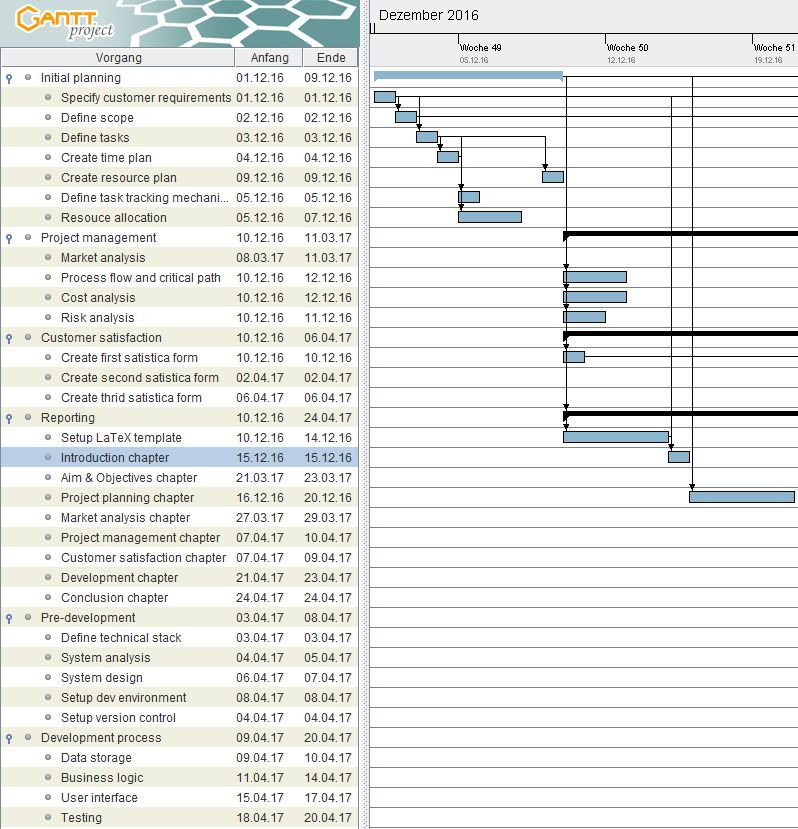
\includegraphics[width=1\textwidth]
     {res/projectPlan/timePlan1.JPG}
     \captionsetup{justification=centering}
  \caption{Final Project Plan}
  \label{fig:project plan}
\end{figure}

Figure \ref{fig:project plan} shows the layout of the GanttProject application
as well as the defined tasks for December 2016 in the chart. It also shows the
aspect that the tasks aren't independent from each other, e.g. the tasks can
only be created if the scope of the project is defined.

\section{Resource Overview}

As soon as the tasks are defined it is necessary to plan the human resources.
The module description states that each team member participates with 100 hours
of work in this project, so the tasks must be distributed consistent. It's the
aim that each team member works on the tasks which are related to their role,
however this can't be achieved 100\% accurately, so it may be the case that the
software architect works on a project management related task.

Because the time period of the project is almost 5 months, the initial planning
tasks are executed in December, while the real project work begins end of
February. This was coordinated with the acceptance of all team members.

The resource overview was also created with the freeware tool GanttProject and
looks as follows:  

\begin{figure}[h!]
  \centering
     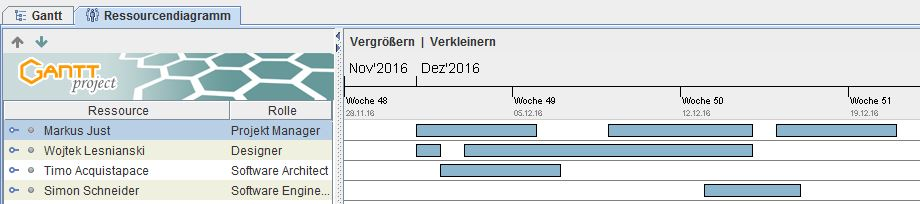
\includegraphics[width=1\textwidth]
     {res/projectPlan/ResourcePlan1.JPG}
     \captionsetup{justification=centering}
  \caption{Resouce Plan December}
  \label{fig:resource plan december}
\end{figure}

\begin{figure}[h!]
  \centering
     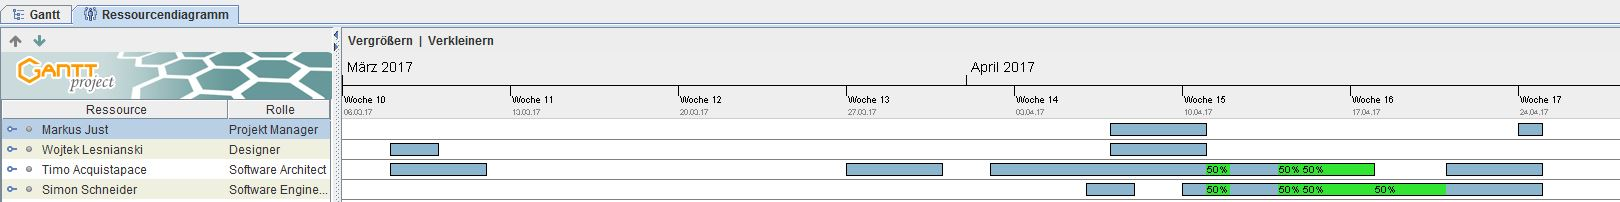
\includegraphics[width=1\textwidth]
     {res/projectPlan/ResourcePlan2.JPG}
     \captionsetup{justification=centering}
  \caption{Resource Plan March / April}
  \label{fig:resource plan march}
\end{figure}

\section{Cost Overview}

After the resource planning is done, it is now possible to look at the costs of
the different work phases as well as the total cost for the resources. Each team
member got a salary of 117\pounds/hour, so the resource cost of the whole
project can be initially calculated with 46.800\pounds (about 100 work hours for
each team member).

The GanttProject tool calculates the costs for each base task and its sub tasks,
which results in the following output:

\begin{table}[h!]
  \centering
\begin{adjustbox}{max width=\textwidth}
\begin{tabular}{|c|c|}
Task&Cost\\
\hline
\rowcolor{lightgray}Initial Planning&8.611\pounds\\
Project Management&9.360\pounds\\
\rowcolor{lightgray}Customer Satisfaction&2.246\pounds\\
Pre-Development&5.242\pounds\\
\rowcolor{lightgray}Development Process&7.114\pounds\\
Reporting&15.023\pounds\\
\rowcolor{lightgray}Total&47.596\pounds\\
\hline
\end{tabular}
\end{adjustbox}
\captionsetup{justification=centering}
  \caption{Cost Overview}
  \label{tab:cost overview}
\end{table}

These overview shows that the estimated costs for executing the defined tasks is
a bit higher than expected, but the difference is not seriously high, so it
isn't much of a problem.

\section{Task Tracking Mechanism}

GanttProject doesn't only provide mechanisms for project planning, it also
provides the possibility to track the current process. This can be achieved by
setting the initial plan as the base plan and after that, the real time spent on
a task can be entered. The GanttProject tool shows the impact on the whole time
plan when a task is finished late/early as it can be seen below:

\begin{figure}[h!]
  \centering
     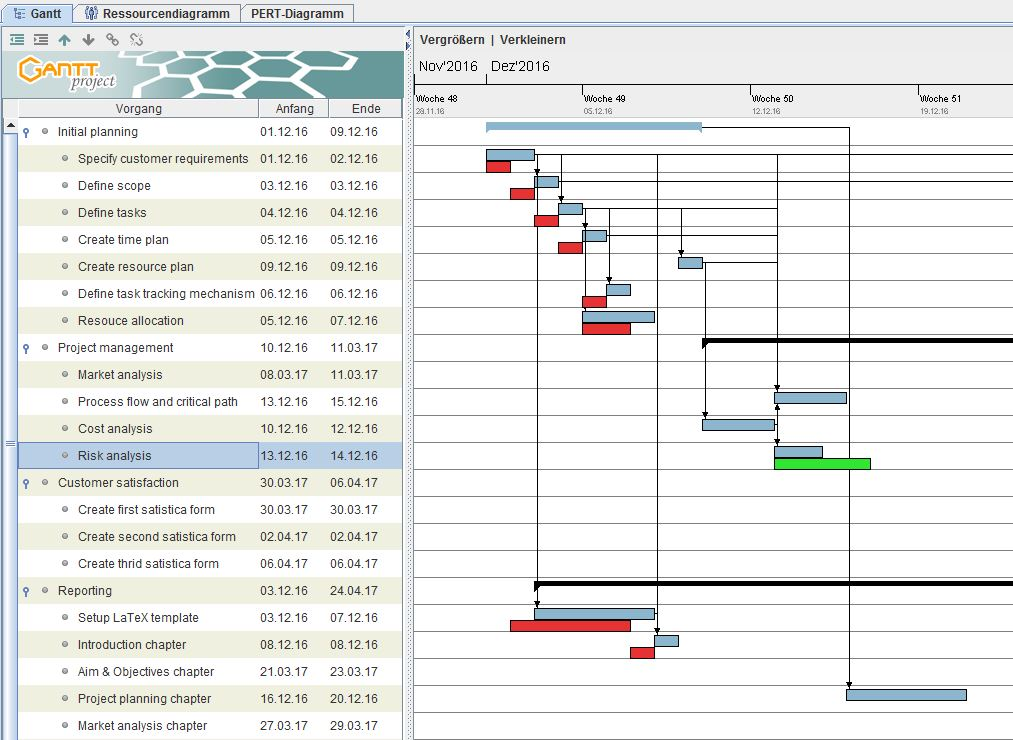
\includegraphics[width=1\textwidth]
     {res/projectPlan/Tracking.JPG}
     \captionsetup{justification=centering}
  \caption{Final Project Plan with Finished Tasks}
  \label{fig:project plan with finished tasks}
\end{figure}

The grey bars show the actual progress of the project. The red/green bars show
the differences to the initial plan. If the bar is red it means the initial
estimated time plan for this task couldn't be followed for this task. If the bar
is green it means this task has been finished earlier than expected.

Each team member should enter the beginning and the duration of the tasks he
finished to make sure that the progression of the project goes forward as it was
planned and the project can be successfully finished until the deadline.

\FloatBarrier

\section{Critical Path}

The ``critical path'' is a planning instrument, which has its origins in the
network plan technology. With its help it is possible to analyse impacts on the
time plan of a project if delays occur during a task execution. The critical
path is the succession of tasks which are interdependent and it indicates the
shortest time needed to finish a project. If one of the tasks belonging to the
critical path is delayed because of some circumstance, the whole project
execution time is delayed as well.

The critical path is useful to analyse which tasks are important and it gives
the possibility to prevent a large delay in finishing the project by
redistribute the resources or move other tasks, which are not part of the
critical path, to the end of the project without further impact on the project
duration.

To visualise the critical path, it is necessary to define the starting dates,
the duration and the dependencies between the tasks. After that each task is
visualised as a process bar and is connected via arrows to other depending
tasks. GanttProject provides the possibility to create a PERT-diagram, which
shows a graphic illustration of a project as a network diagram. Unfortunately
GanttProject isn't able to create a clear PERT-chart which can be pasted here,
so the complete diagram can be found in the appendix:

\textbf{\color{red}{des PERT-Diagramm vom Markus fehlt noch -.-}}
